% 几何矢量

我们来回顾高中学的\bb{几何矢量}, 以下简称为“矢量”. 要强调的是, 矢量的存在与坐标系无关, 可以将其想象成空间中的一些有长度有方向的箭头. 我们对它的位置不感兴趣, 所有长度和方向相同的矢量都视为同一矢量. 本书中矢量用正黑体表示, 如 $\vec a$. 在手写时, 可以在字母上方加箭头表示, 如 $\overrightarrow{a}$. 特殊地, 如果一个矢量的长度等于 1, 那么它就是一个\bb{单位矢量}, 本书中在矢量上面加上 “\^{}” 符号表示单位矢量, 如 $\uvec a$. 为了与矢量区分, 我们把单个的实数或复数称为\bb{标量}.

\subsection{矢量的加法}
如\autoref{GVec_fig1},两个矢量相加, 既可以使用平行四边形法则, 也可以用三角形法则. 若有多个矢量连续相加, 可以分别把它们首尾相接, 结果就是由起点指向终点的矢量. 容易证明矢量的加法满足加法交换律 $\vec A + \vec B = \vec B + \vec A$, 结合律 $(\vec A + \vec B) + \vec C = \vec A + (\vec B + \vec C)$.
\begin{figure}[ht]
\centering
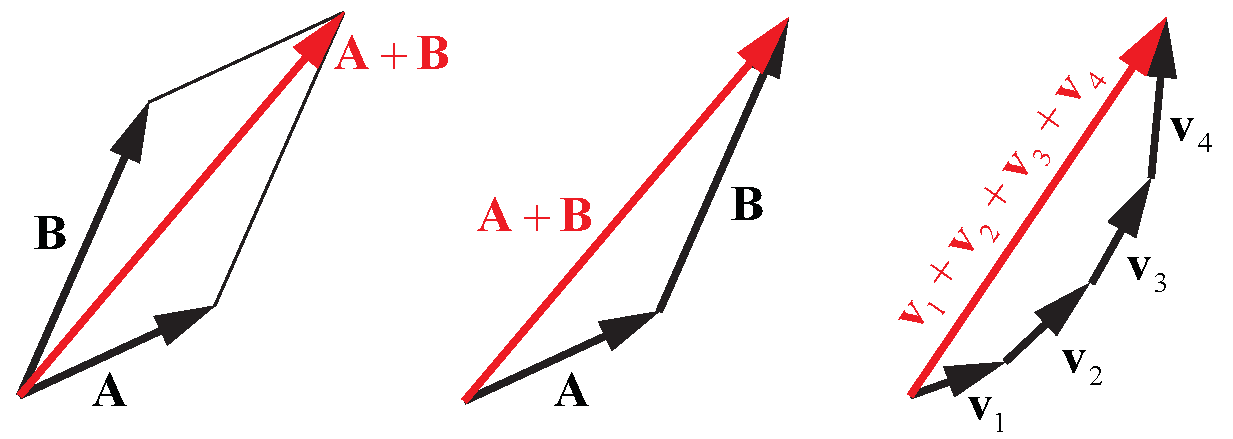
\includegraphics[width=10.5cm]{./figures/GVec1.pdf}
\caption{矢量的加法} \label{GVec_fig1}
\end{figure}

\subsection{矢量的数乘\ 共线}
如\autoref{GVec_fig2}, 一个矢量与一个正实数相乘, 则方向不变, 把长度乘以这个实数. 若这个数是负数, 则把矢量取反方向再把长度乘以这个实数数的绝对值即可.若 $\lambda, \mu$ 表示实数, 容易证明分配律 $\lambda(\vec A + \vec B) = \lambda\vec A + \lambda\vec B$ 和 $(\lambda+\mu)\vec A = \lambda\vec A + \mu\vec A$, 结合律 $\lambda(\mu\vec A) = (\lambda\mu) \vec A$.
\begin{figure}[ht]
\centering
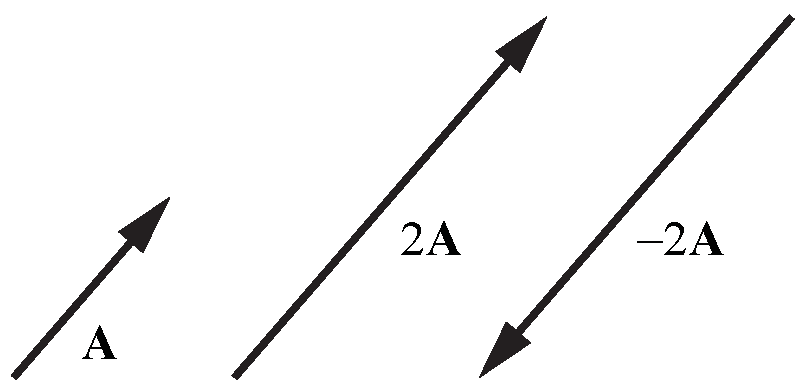
\includegraphics[width=6.5cm]{./figures/GVec2.pdf}
\caption{矢量的数乘} \label{GVec_fig2}
\end{figure}

如果两个矢量的关系可以用 $\vec A = \lambda\vec B$ 表示, 那么它们就是\bb{共线}的. 共线的充分必要条件\upref{SufCnd}是, 两矢量方向相同或相反.

\subsection{矢量的线性组合}
把若干矢量 $\vec v_i$ 分别与若干实数 $c_i$ 相乘再相加就得到了这些矢量的一个\bb{线性组合}
\begin{equation}
\sum_i^N c_i \vec v_i = c_1\vec v_1 + c_2\vec v_2 +\dots +c_N \vec v_N
\end{equation}

\subsection{线性相关\ 线性无关}
如果存在至少一组不全为零系数 $c_i$ 使几个矢量的线性组合等于零, 这些矢量就被称为\bb{线性相关}的
\begin{equation}\label{GVec_eq2}
\sum_i^N c_i \vec v_i = \vec 0
\end{equation}
这是因为对于任何一个不为零的项 $j$, 矢量 $\vec v_j$ 都可以表示为其他矢量的线性组合. 只需把上式除以 $c_j$ 即可
\begin{equation}\label{GVec_eq3}
\vec v_j = \sum_{i \ne j}\frac{c_i}{c_j} \vec v_i
\end{equation}
如果不存在这样的系数, 这些矢量就是\bb{线性无关}的. 

\subsection{基底\ 矢量空间\ 坐标}
沿一条直线的所有矢量都是共线的, 所以在一条直线上最多不超过一个矢量线性无关, 所有这些共线的矢量以及它们的加法和数乘运算组成一个\bb{一维矢量空间}\footnote{注意这里并没不打算给出矢量空间的一般定义, 只是说“是一个矢量空间”.}. 一个平面上的所有矢量以及它们的加法和数乘运算, 组成一个\bb{二维矢量空间}, 二维矢量空间中最多只能找到两个线性无关的矢量. 三维矢量空间同理. 

$N$ 维空间中的任意一组线性无关的 $N$ 个矢量 $\vec \beta_1\dots \vec \beta_N$ 可以作为一组\bb{矢量基底}, 记为 $\{\vec \beta_i\}$. 如果在这组基底中加入该空间中任意一个矢量 $\vec v$, 这组 $N+1$ 个矢量必定线性相关(否则空间就是 $N+1$ 维的), 即存在不全为零的实数 $c_1\dots c_{N+1}$ 使下式成立
\begin{equation}
\sum_{i=1}^N c_i \vec \beta_i + c_{N+1} \vec v = \vec 0
\end{equation}
我们还可以得知 $c_{N+1}$ 必不为零(反证法:如果 $c_{N+1} = 0$, 则可得出基底 $\{\vec \beta_i\}$ 线性相关, 不成立), 所以由\autoref{GVec_eq3} 可知 $\vec v$ 可用 $\{\vec \beta_i\}$ 的线性组合表示. 令 $x_i = -c_i/c_{N+1}$, 该空间中任意矢量 $\vec v$ 都有
\begin{equation}\label{GVec_eq5}
\vec v = \sum_{i=1}^N x_i \vec \beta_i
\end{equation}
这里的 $x_i$ 就是矢量空间中\bb{坐标}的定义.

我们可以用反证法证明坐标的唯一性. 假设有两组不全相同的 $x_i$ 都可以是上式成立, 分别记为 $x_i$ 和 $y_i$. 那么分别代入上式再把两式相减得到
\begin{equation}
\sum_{i=1}^N (x_i-y_i) \vec \beta_i = \vec 0
\end{equation}
由于 $(x_i-y_i)$ 不全为零, 得到基底 $\{\vec \beta_i\}$ 线性相关, 而这是不可能的.证毕.

\subsection{坐标的运算}
我们常常把一个矢量的坐标写成一个\bb{代数矢量}, 如
\begin{equation}\label{GVec_eq7}
\vec v = \pmat{x\\y\\z}_{\{\vec\beta_i\}}
\end{equation}
在列矢量的右下角声明基底是较为严谨的做法, 但为了书写简洁, 在不至于混淆的情况下我们可以将其省略. 另外在正文中, 为了节约空间, 我们将\autoref{GVec_eq7} 记为 $\vec v = (x, y, z)_{\{\vec\beta_i\}}\Tr$(见“矩阵\upref{Mat}” \autoref{Mat_eq2} ), 同样, 我们时常省略 $\{\vec\beta_i\}$.

当我们说两个矢量\bb{相等}时, 同一基底下两矢量的坐标全都需要相等. 若已知两矢量在不同基底下的列矢量, 则需要先将它们变换到同一基底下再判断是否相等.

以上介绍的加法和数乘都有对应的坐标运算. 由\autoref{GVec_eq5} 及矢量加法和数乘的交换律和结合律得
\begin{equation}\label{GVec_eq8}
\vec v_1 + \vec v_2 = \pmat{x_1\\y_1\\z_1}_{\{\vec\beta_i\}} + \pmat{x_2\\y_2\\z_2}_{\{\vec\beta_i\}} = \pmat{x_1 + x_2\\y_1 + y_2\\z_1 + z_2}_{\{\vec\beta_i\}}
\end{equation}
\begin{equation}\label{GVec_eq9}
\lambda \vec v = \lambda\pmat{x\\y\\z}_{\{\vec\beta_i\}} = \pmat{\lambda x\\\lambda y\\\lambda z}_{\{\vec\beta_i\}}
\end{equation}

要特别注意的是, 当定义了多组基底时, 只有基底相同的两个列矢量按照\autoref{GVec_eq8} 相加才有意义.

\rentry{矢量的点乘\upref{Dot}, 正交归一基\upref{OrNrB}, 矢量的叉乘\upref{Cross}}




